\section{Results}
\label{sec:results}

We demonstrated that our improvised system is highly effective against Apple's CAPTCHA system resulting in a 22\% increase in accuracy for Google UK solver. This yielded us our best solver for Apple with 66\% accuracy. We got a final accuracy of 60\% when testing with 1000 CAPTCHAs. It also  performed well with Telerik's CAPTCHA system, improving the accuracy of IBMWatson US Accent solver from 64\% to 88\%. When tested with 1000 CAPTCHAs, we got an accuracy of 90\%. All the results of our experiments are given in Figure 8 .\newline

We observed that denoising helped all CAPTCHA systems except reCAPTCHA and Securimage. The quality of the audio file decreased after denoising for reCAPTCHA because the background noise that was added was of very short-length and difficult to remove. In case of Securimage, there was too much background noise and the amplitude of the background noise was as high was the actual signal. Thus removing it was very difficult. Also, on the whole, Wit.ai solver performed better before denoising than after it. \newline

Microsoft Live was hard to crack because they do not have a corpora of words that they construct audio challenges from, unlike others that give out digits, alphabets, NATO words or a combination of any of these. We also showed that our attack was least effective against Securimage, which uses background noise to mask the audio.\newline

\begin{figure}[t]
   \centering
   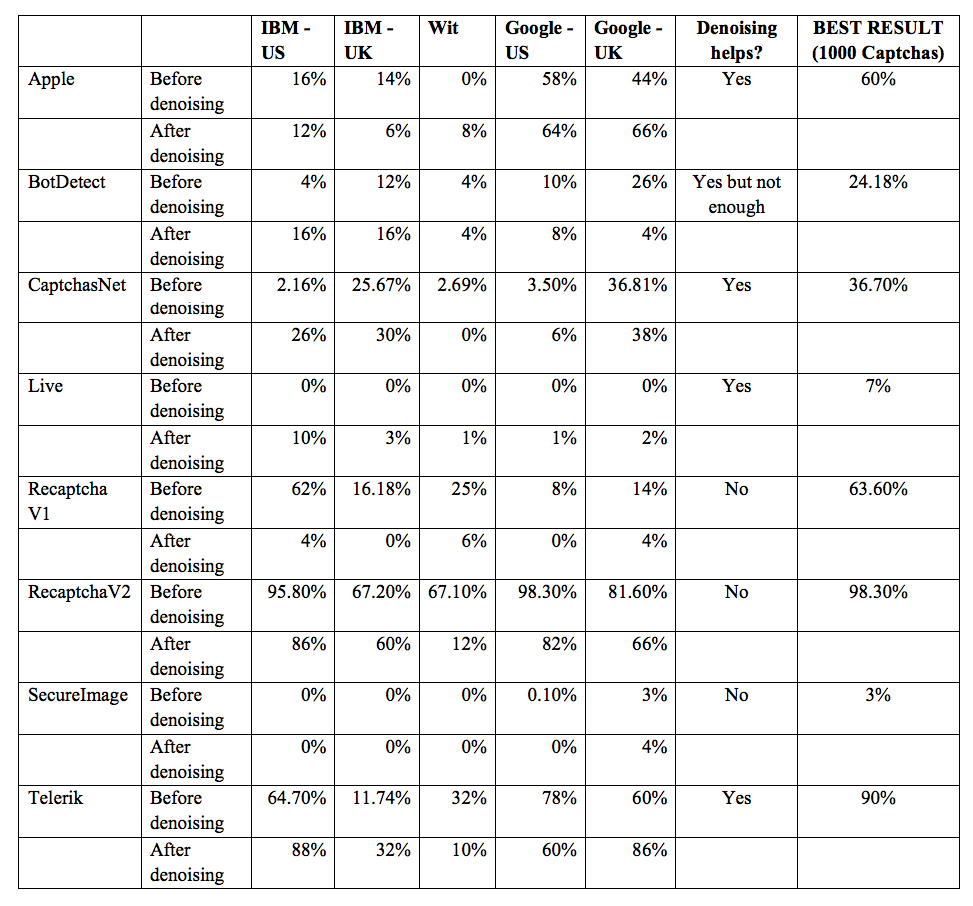
\includegraphics[width=\columnwidth]{figures/results4.jpg}.
   \caption{Results - Accuracy of our solvers with all 8 CAPTCHA systems, after denoising.}
   \label{fig:results2}
\end{figure}


